\chapter{Uso de refugios}
 
\chapterquote{In retrospect, Euler's unintended message is very simple: Graphs or networks have properties, hidden in their construction, that limit or enhance our ability to do things with them.}{Albert-László Barabási, 1982}
 
Para varias especies los refugios son fundamentales para la protección ante depredadores y  condiciones climáticas adversas, especialmente para animales ectotérmicos, como las tortugas que dependen de fuentes externas para la obtención de calor. En especies relativamente solitarias, es esperable que los individuos pasen un tiempo considerable solos en los refugios o tengan pocos encuentros directos fuera de la época de apareamiento \cite{bipartitasTortusPaper}. Ejemplos de estas especies incluyen a los mapaches, zorros rojos, orangutanes y algunas especies de abejas, avispas y murciélagos. Para estas poblaciones de animales salvajes, monitorear y entender estos refugios puede ayudar a establecer patrones sociales de los individuos.
 
En distintos campos cercanos a la zona de medición (San Antonio Oeste, provincia de Río Negro) están introduciendo ganado en el habitat de las tortugas, por lo tanto es importante entender si esta perturbación presenta una amenaza para la integridad de los refugios. Entender el patrón de movimiento  de las tortugas, junto con las características geográficas de los refugios más usados es de fundamental importancia para el establecimiento de políticas de conservación.
 
\section{Refugios en el mapa}
Para determinar el refugio donde pasó la noche la tortuga se tomaron dos criterios, uno para cada una de las metodologías de medición. Para la metodología de tortugómetro se tomó el último punto registrado de la tortuga en un día de medición y se pidió la condición que haya sido tomado después de las 20 horas. En base a las anotaciones de campo tomadas por el grupo, las tortugas generalmente  se encontraban en el refugio cuando quitaban los tortugómetros después de este horario. A este punto nuevo se le asigna una etiqueta de refugio y un enlace a la tortuga que pasó la noche en ese refugio. A medida que se añade otro refugio, primero se verifica que presente una distancia mayor a 20 metros con todos los otros refugios etiquetados. En caso de que la distancia sea menor de 20 metros al refugio 1 (por ejemplo) se dice que la tortuga estuvo en el refugio 1.
                 
Para los datos tomados por los i-gotU, se decidió mirar primero las distancias recorridas entre el último punto medido (21:00 horas) de algún día monitoreado y el primer punto del día siguiente (6:00 horas). También se miraron las distancias entre el primer punto de algún día de monitoreo con el segundo punto (6:00 horas y 6:15 respectivamente). En la Fig. \ref{fig:distancias} se muestran los histogramas de las distancias para ambos casos. Se observa que entre el último punto de la noche y el primero de la mañana distancias mayores a 20 metros son muy probables, con varias mediciones de distancias del orden de los 50 o 100 metros, lo que nos diría que la tortuga no se encuentra aún en el refugio a las 21 horas. En cambio, entre el primer punto del día y el segundo punto, las distancias menores a 20 metros son las más probables, lo que nos diría que la tortuga todavía no abandonó el refugio entre las 6:00 y las 6:15, a excepción de algunos pocos casos donde tenemos distancias del orden de los 50 m. Por ese motivo, para los datos de los i-gotU se decidió tomar el primer punto del día como la posición del refugio y se siguió el mismo procedimiento que con los tortugómetros para agregar etiquetas a los refugios. En función de este resultado, para próximas campañas se decidió mantener las mediciones del i-gotU entre las 21:00 y las 6:00 horas, pero disminuyendo la frecuencia de muestreo.
 
 
\begin{figure}[ht]
    \begin{center}
        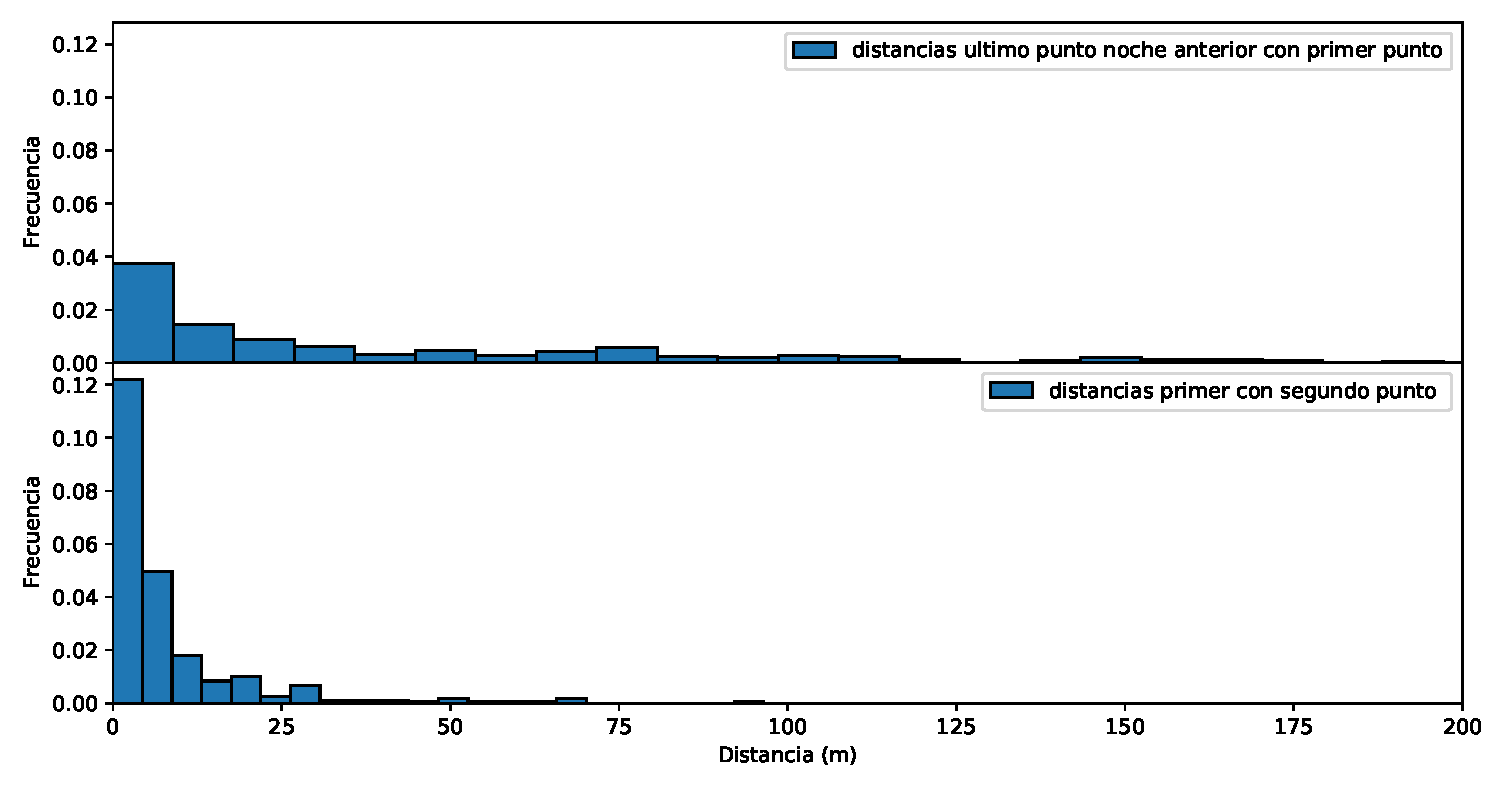
\includegraphics[width=1.4\imsize]{Chap3/Distancias_primer_ult_con_deteterminar_criterio_ref.pdf}
        \caption[Histogramas de las distancias entre los puntos de los datos de i-gotU.]{ Histogramas de las distancias entre los puntos de los datos de i-gotU. Arriba se muestra la distancia entre el último punto del día anterior y el primer punto del día siguiente. Abajo se muestra la distancia entre el primer punto del día y el segundo punto del día.}
        \label{fig:distancias}
        \end{center}
\end{figure}
 
Se graficaron los refugios encontrados en un mapa utilizando la librería Folium. Los mapas fueron guardados en formato html para el fácil acceso a los mismos y al clickear en un refugio sobre el html aparece un cartel con las tortugas que pasaron la noche en el mismo. En las Fig. \ref{fig:refus_campanas_con_labels} y \ref{fig:refus_igotu_labels} se muestran los mapas de los refugios encontrados para los datos de las campañas y los datos de i-gotU respectivamente.
 
 
\begin{figure}[ht]
    \begin{center}
        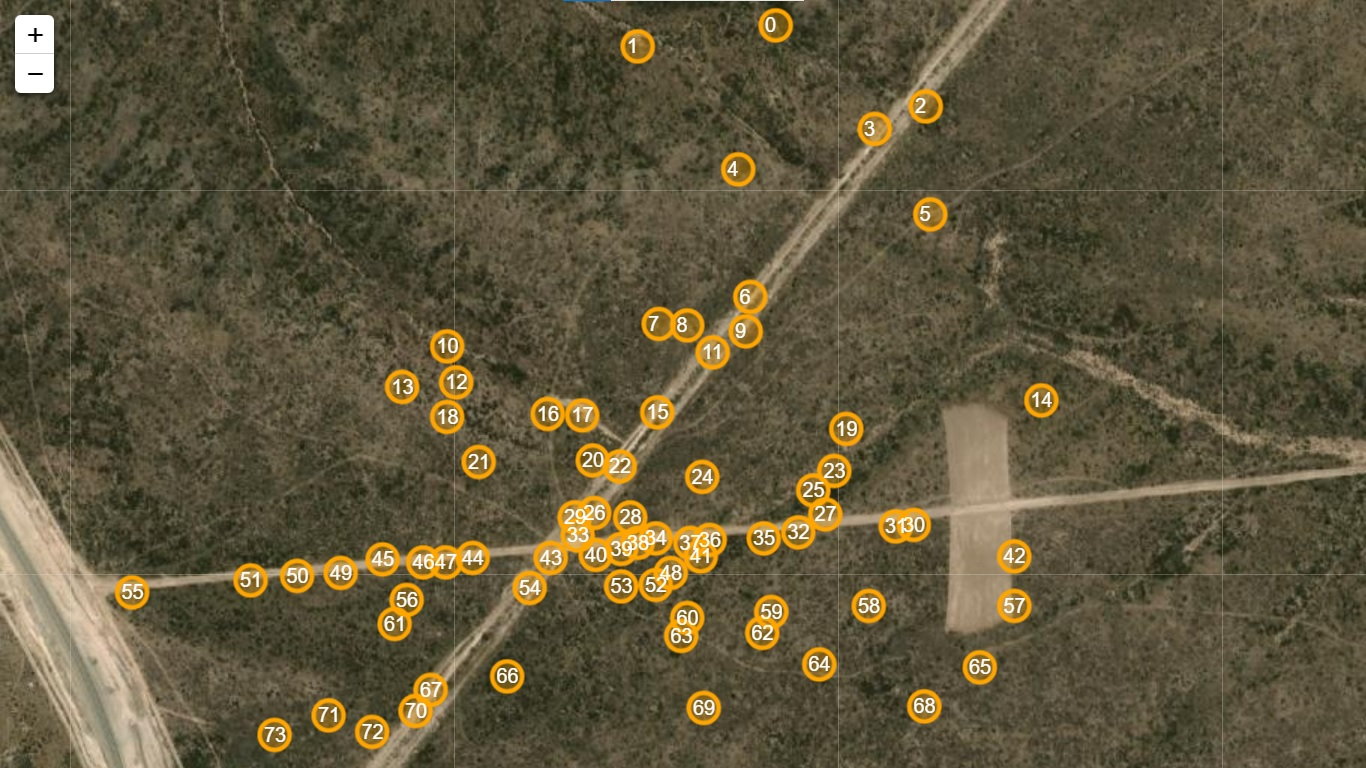
\includegraphics[width=\imsize]{Chap3/map_refugies_with_labels.jpg}
        \caption{Distribución geográfica de los refugios encontrados para los datos provenientes de las campañas.}
        \label{fig:refus_campanas_con_labels}
       
        \end{center}
\end{figure}
 
\begin{figure}[ht]
    \begin{center}
        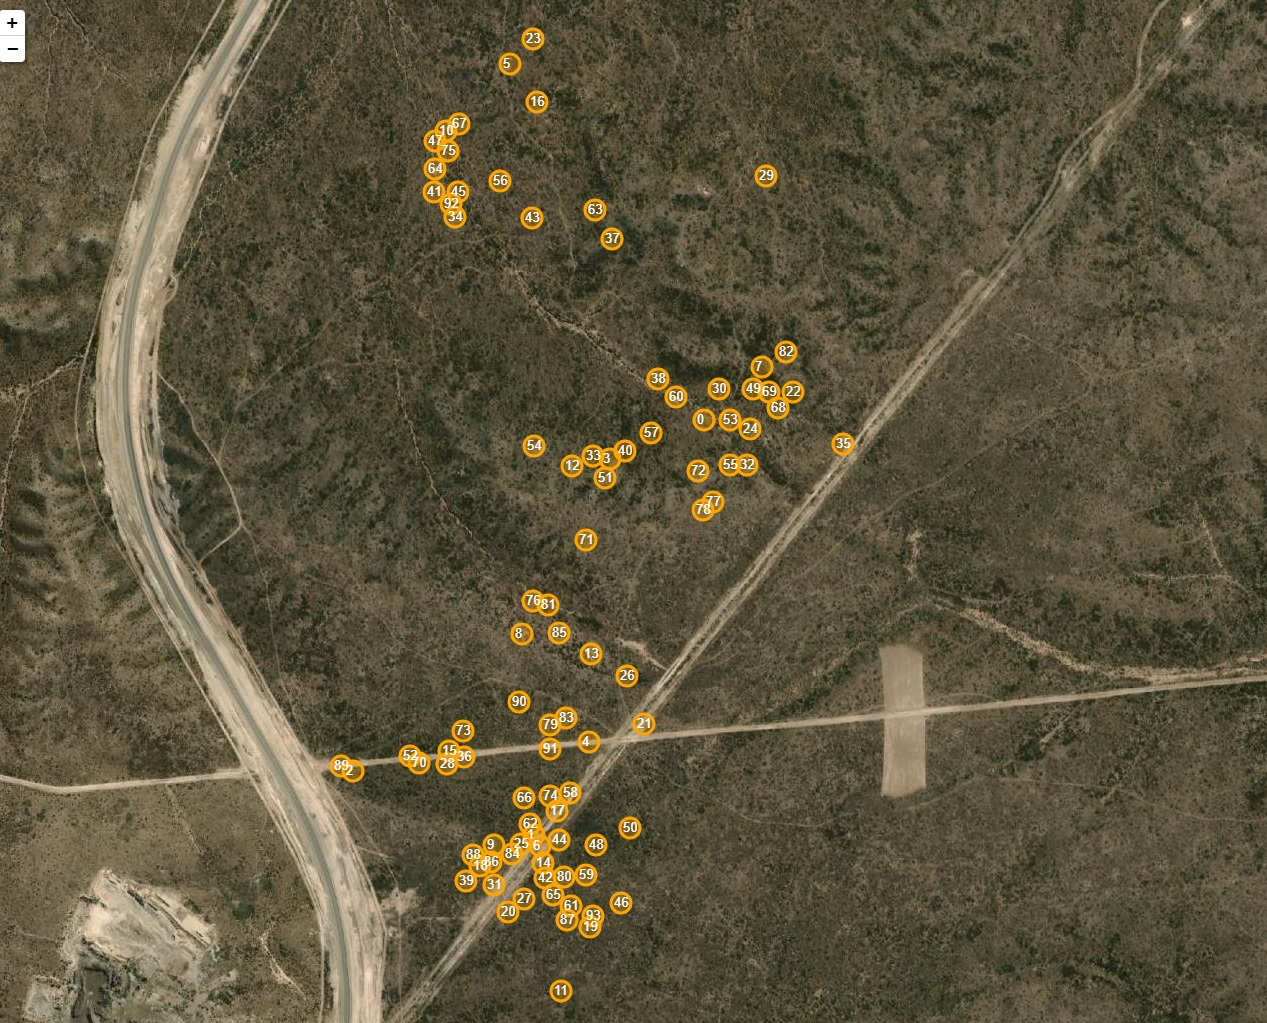
\includegraphics[width=\imsize]{Chap3/map_refugies_with_labels_IGOTo.jpg}
        \caption{Distribución geográfica de los refugios encontrados para los datos provenientes de los datos de i-gotU.}
        \label{fig:refus_igotu_labels}
       
        \end{center}
\end{figure}
 
En base a observaciones directas de campo \cite{Erika}, se observaron ciertos machos en distintas zonas de medición, en particular para la época de apareamiento. Estas observaciones aisladas nos llevaron a pensar que es posible que  tortugas macho tengan una distribución de refugios más amplia en el espacio que tortugas hembra.  Para poner a prueba esta hipótesis se definieron dos métricas: centro de masa de refugios y distancia media entre refugios. El centro de masa se define como:
\begin{center}
   
 
$$X_{centro}= \sum^{N -1}_{n=0} \frac{i_{n} X_n}{I_{totales}}.$$
\end{center}
Donde $I_{totales}$ es la cantidad de noches donde se registró que la tortuga durmió en un refugio (depende de cada tortuga), $X_n$ es la coordenada $X$ del refugio $n$, $i_{n}$ es la cantidad de noches que la tortuga durmió en el refugio $n$ y $N$ la cantidad de refugios totales.  Esta cantidad se calcula para todas las tortugas.
Partiendo de $X_{centro}$, la distancia media  espacial de los refugios se calcula como:
$$D = \sum^{N -1}_{n=0} \frac{|X_n i_n - X_{centro}|}{I_{totales}}.$$
\label{eq:distancia_media_refugios}
El valor de $D$ da una idea de la extensión en el espacio de los refugios de una dada tortuga. Cuanto mayor es el valor de $D$, más dispersos estarán los refugios en el espacio. Esta métrica fue calculada para todas las tortugas y  promediada para  machos y hembras. Se encontró para los machos $\overline{D}_m =  (128\pm66)\,\text{m}$ y para las hembras     $\overline{D}_h = (122\pm82)\,\text{m}$. Es decir que no se encontraron diferencias significativas en la distribución espacial de refugios  entre machos y hembras.
\section{Refugios más usados y caminos tomados}
Dentro de los refugios que utiliza una tortuga, se encontraron refugios preferidos, es decir refugios que fueron visitados recurrentemente. Para observar esto se decidió graficar la acumulada de noches pasadas en un refugio para los refugios más utilizados por una tortuga, y así poder visualizar la cantidad de noches que pasó en el refugio preferido y los días donde volvió al mismo. Esto se realizó solo para los datos provenientes de los i-gotU, ya que se contó con una gran cantidad de días consecutivos de medición (Fig. \ref{fig:refugios_preferidos}).
\begin{figure}[ht]
    \begin{center}
        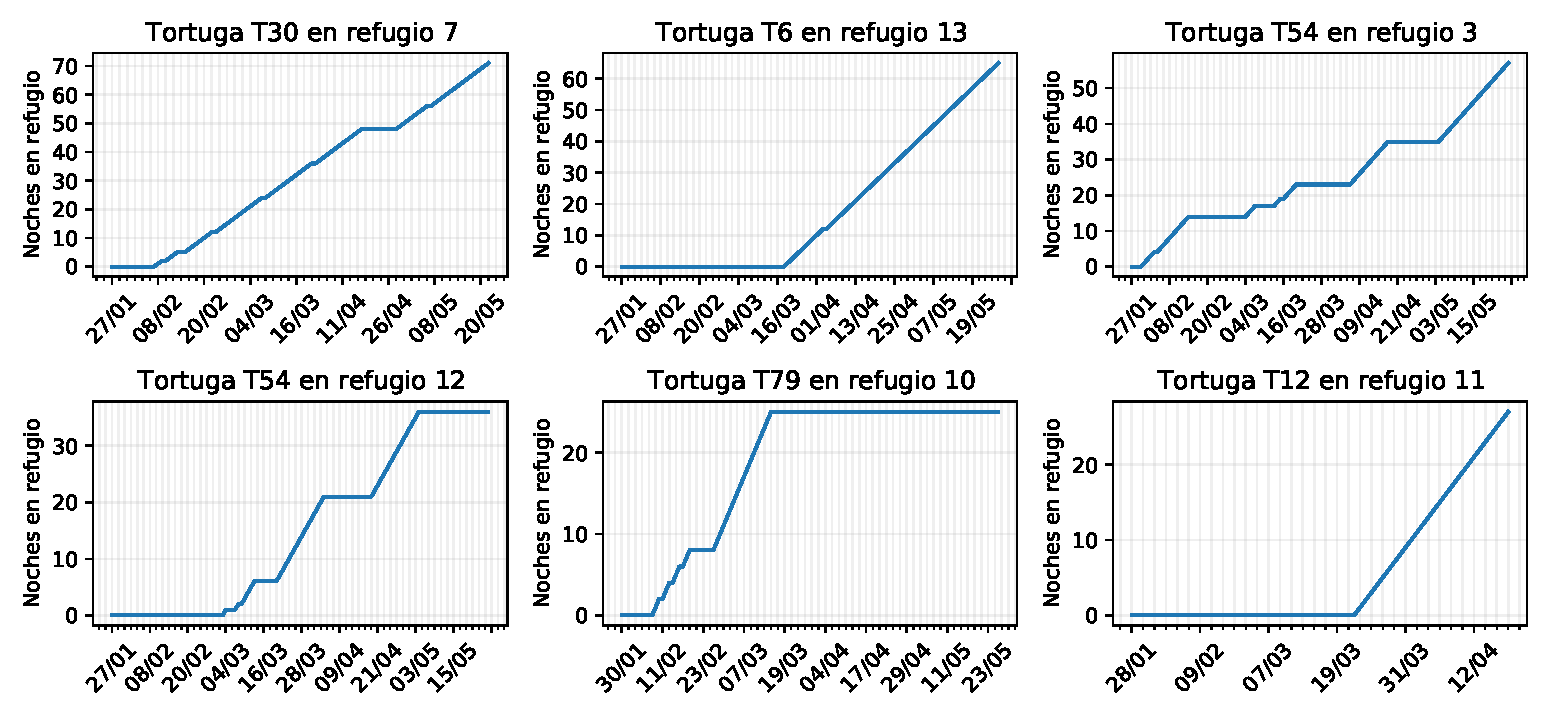
\includegraphics[width=1.4\imsize]{Chap3/acumulada_de_noches_en_refmasUsados_espanol.pdf}
        \caption[Acumulada de noches pasadas en los refugios preferidos.]{Acumulada de noches pasadas en los refugios preferidos para distintas tortugas monitoreadas por los i-gotU de enero 2022 a mayo 2022.}
        \label{fig:refugios_preferidos}
       
        \end{center}
\end{figure}
Se observa en la Fig. \ref{fig:refugios_preferidos} que las tortugas tienen un refugio preferido donde pasan la mayor parte de las noches monitoreadas (donde la recta tiene pendiente es positiva). Sin embargo, también se observó que algunas tortugas tienen varios refugios preferidos, como es el caso de la tortuga T54. En las tortugas T30, T54, T6 y T79, se registraron días donde cada tortuga decidió pasar la noche en otro refugio (línea horizontal) para después volver a su refugio preferido (recta con pendiente positiva).
 
Para visualizar estas rutas entre refugios y la preferencia relativa entre ciertos refugios, se realizaron mapas con la librería Folium donde se graficaron los refugios con círculos de tamaño proporcional a la cantidad de noches que la tortuga pasó en el refugio y con conexiones entre refugios ilustrando las rutas tomadas. Es decir si la T54 pasó una noche en el refugio 12 y la noche siguiente en el refugio 3, habrá una línea entre el refugio 12 y el refugio 3 en el mapa. En la Fig. \ref{fig:ruta_refus_T54} se muestra un ejemplo de este tipo de mapa para la tortuga T54.
 
\begin{figure}[ht]
    \begin{center}
        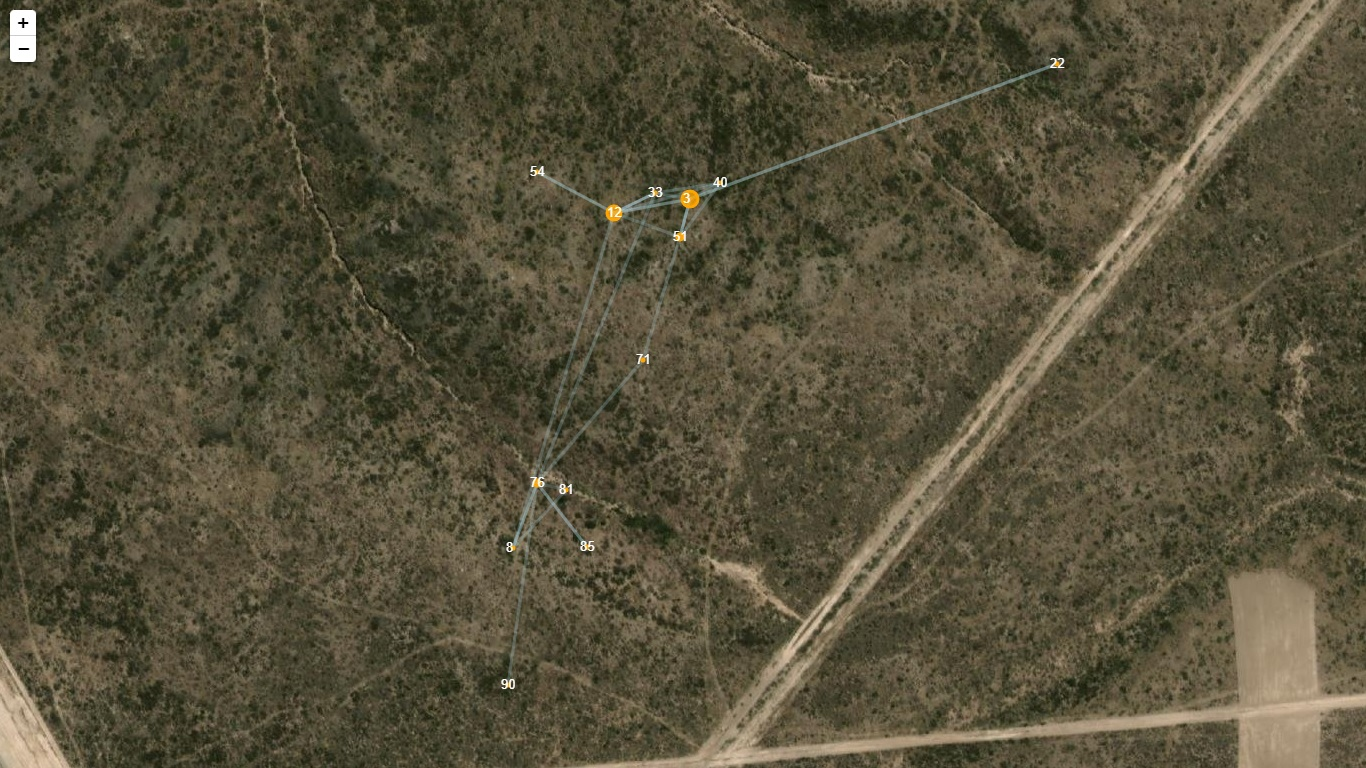
\includegraphics[width=\imsize]{Chap3/refugies_path_for_t54.jpg}
        \caption[Caminos tomados entre refugios para la tortuga T54.]{Caminos tomados entre refugios para la tortuga T54. El tamaño de nodo refugio es proporcional a la cantidad de noches que pasó la tortuga en el mismo. Una conexión entre un par de nodos refugio aparece solo si pasó una noche en el refugio de origen y la noche siguiente en el refugio de destino. Al cliquear sobre un nodo refugio se puede ver la cantidad de noches que pasó la tortuga en el mismo.}
        \label{fig:ruta_refus_T54}
       
        \end{center}
\end{figure}
Haber encontrado preferencia por ciertos refugios abre distintas preguntas: ¿Qué características comparten estos refugios preferidos? ¿Siguen recurriendo a estos refugios en distintas épocas del año u otros años?  Responder estas preguntas podría ayudarnos a entender el rol de la memoria en esta especie de reptiles y a plantear medidas de conservación de la especie. En futuras campañas de medición se espera poder entender más sobre estos refugios preferidos.
 
 
 
%hasta aca corregido
\section{Redes bipartitas de refugios}
Se armaron redes bipartitas con nodos refugio y nodos tortuga. En este tipo de redes, los nodos refugio solo están conectados con nodos tortuga y las conexiones indican que esa tortuga usó ese refugio. Partiendo de todas las etiquetas de refugios con las tortugas que pasaron noche en ese refugio, se armaron las redes bipartitas para los datos tomados por los tortugómetros y los datos tomados con los i-gotU, Figs. \ref{fig:red_bipartita_refus_campanas} y \ref{fig:red_bipartita_refus_igotu} respectivamente.
 
\begin{figure}[ht]
    \begin{center}
        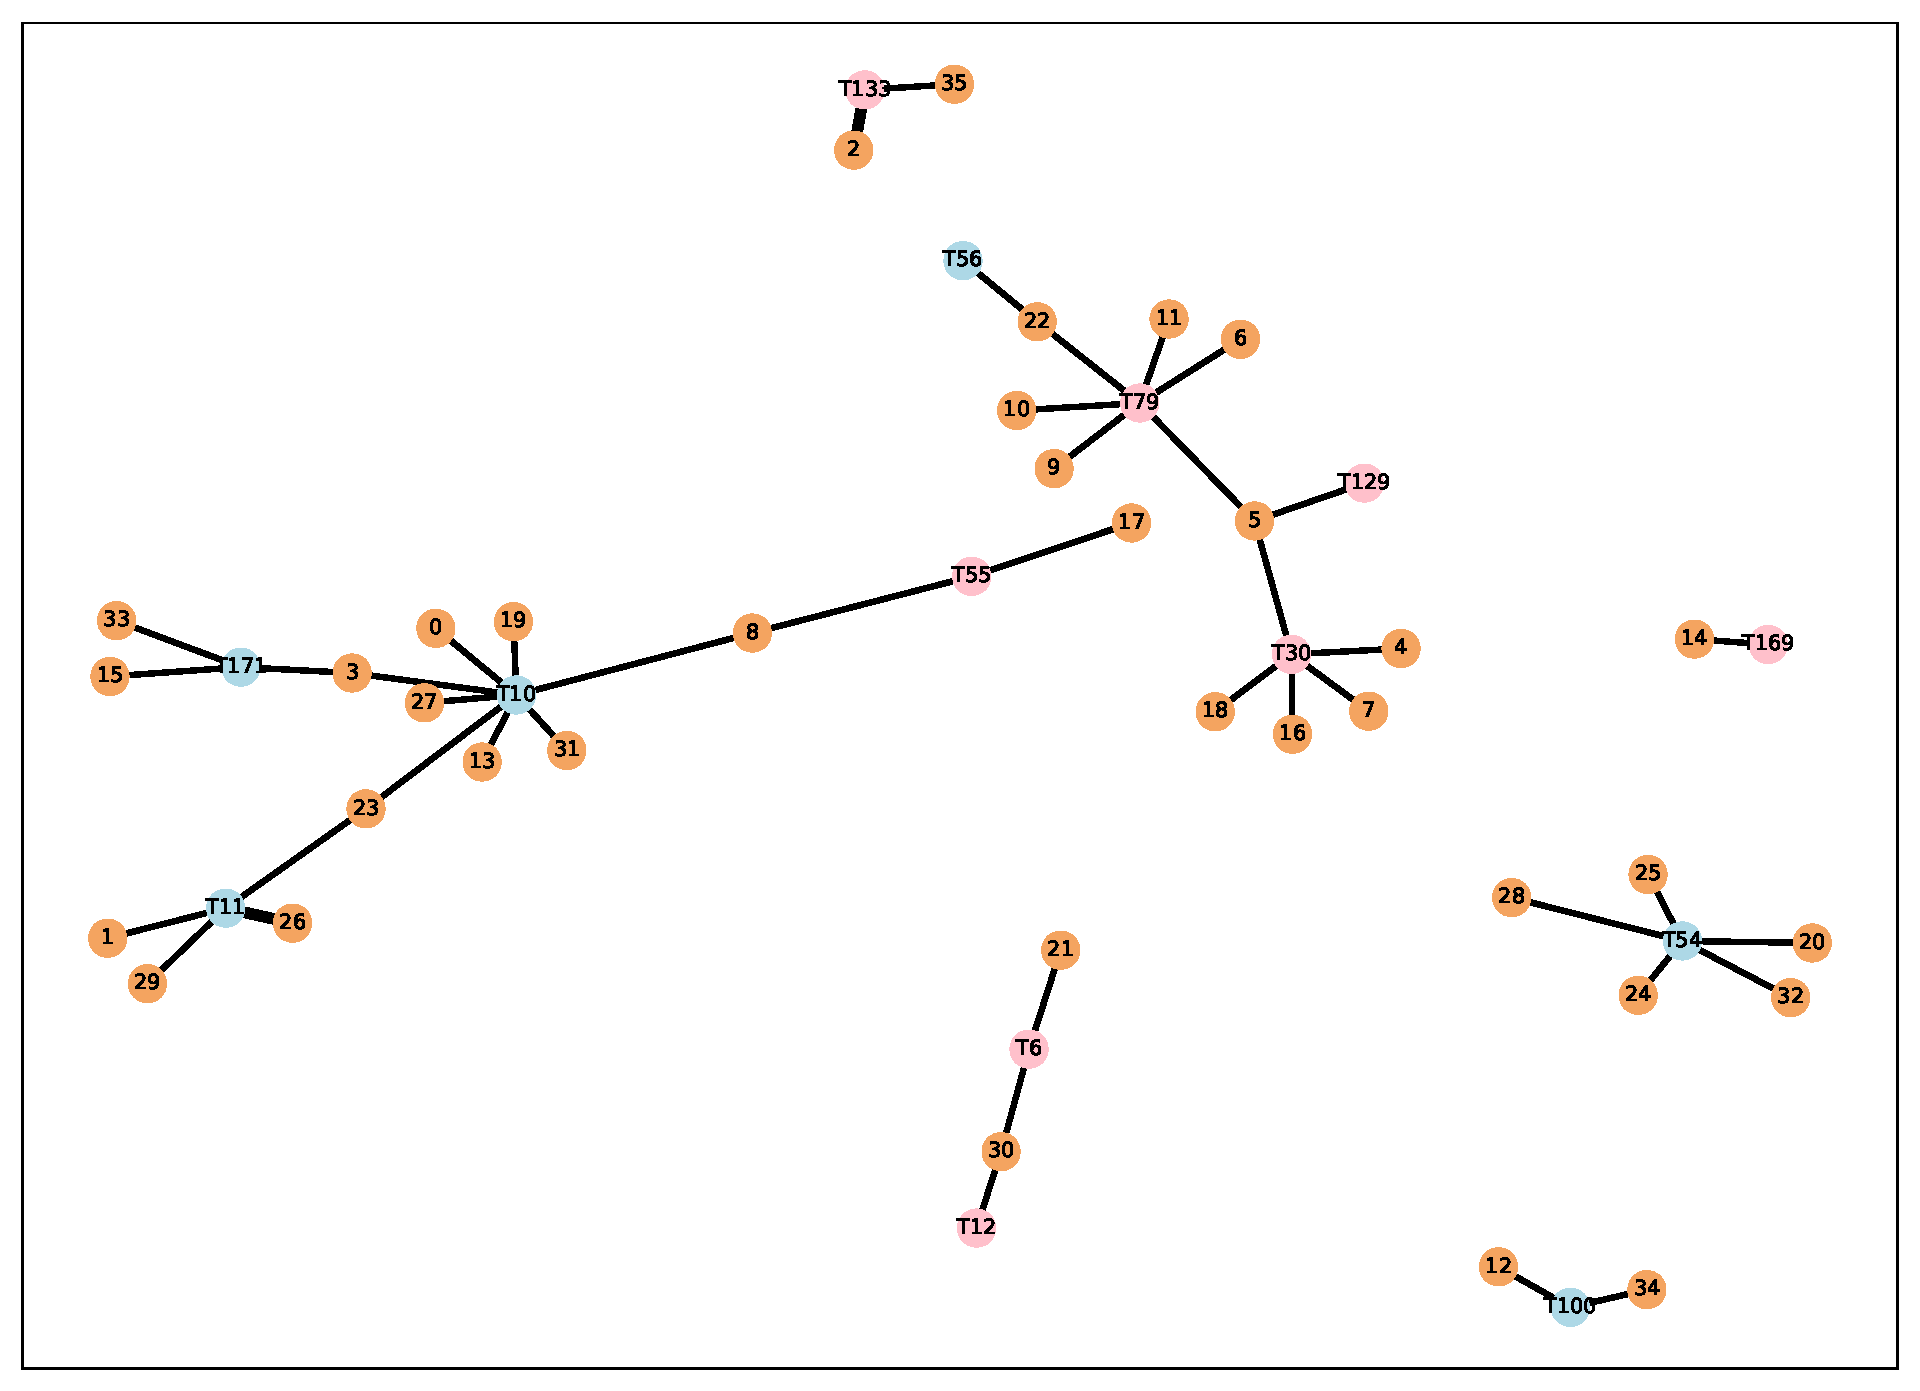
\includegraphics[width=\imsize]{Chap3/RedBipartita_deRefugios_corregida_campanas_2300.pdf}
        \caption[Red bipartita de refugios para los datos de los tortugómetros.]{Red bipartita de refugios para los datos de los tortugómetros. Las distancias relativas entre nodos y el grosor del enlace es dependiente de la cantidad de noches que una  tortuga pasó en el refugio. }
        \label{fig:red_bipartita_refus_campanas}
       
        \end{center}
\end{figure}
 
\begin{figure}[ht]
    \begin{center}
        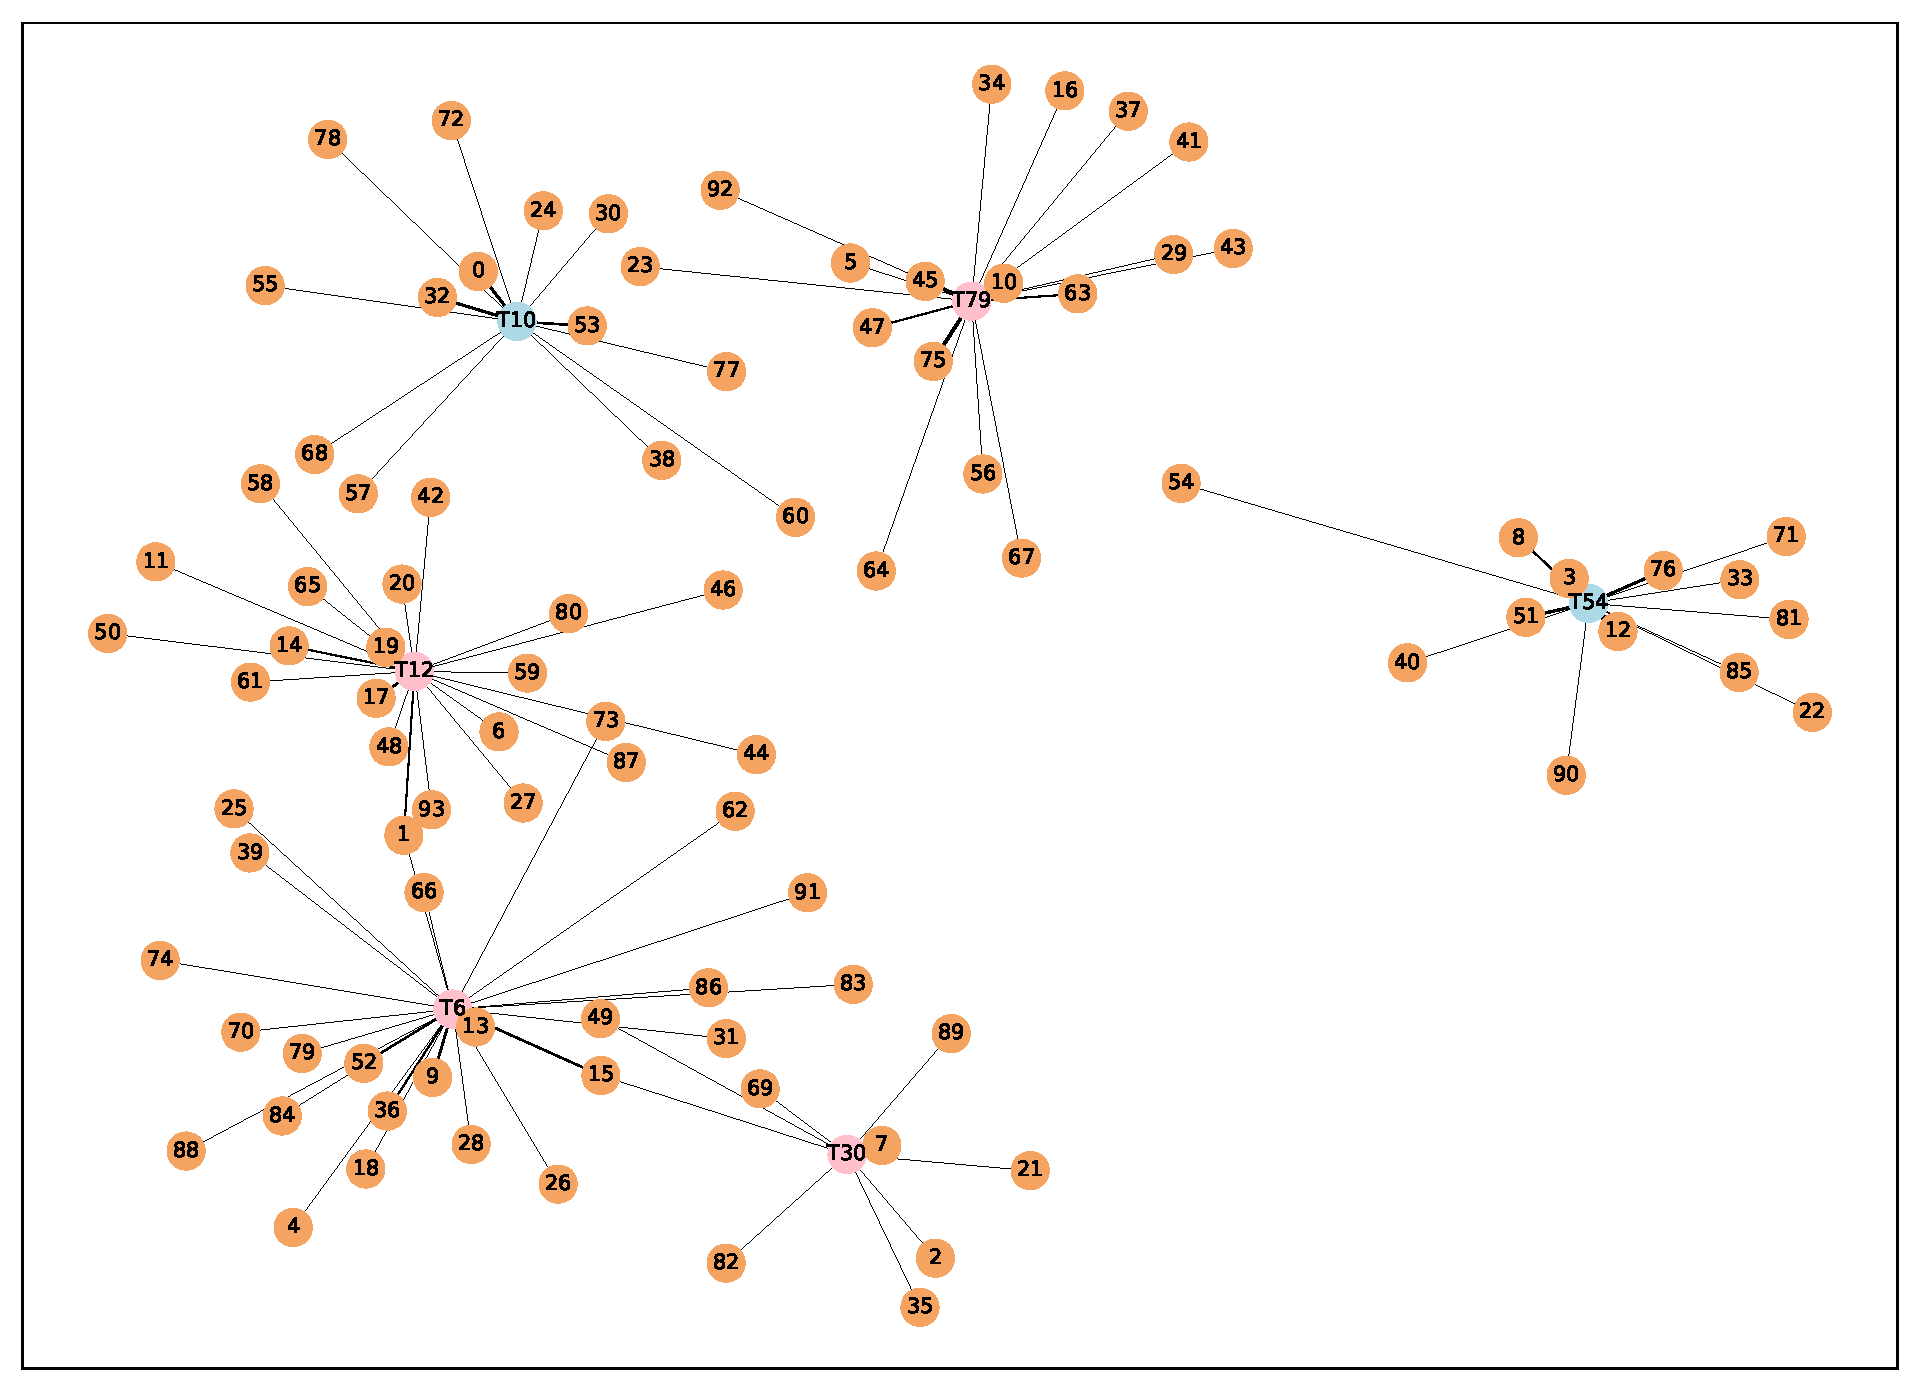
\includegraphics[width=1.3\imsize]{Chap3/RedBipartita_deRefugios_IGOTO.pdf}
        \caption[Red bipartita de refugios para los datos de los i-gotU.]{Red bipartita de refugios para los datos de los i-gotU. Las distancias relativas entre nodos y el grosor del enlace es dependiente de la cantidad de noches que una  tortuga pasó en el refugio. }
        \label{fig:red_bipartita_refus_igotu}
       
        \end{center}
\end{figure}
En la Figs. \ref{fig:red_bipartita_refus_campanas} y \ref{fig:red_bipartita_refus_igotu}, se observan refugios compartidos entre dos y tres tortugas.  En base a este resultado, se decidió buscar la probabilidad de que dos nodos tortuga estén conectados en la red de encuentros (Figs. \ref{fig:redInteraccion20mincampanas} y \ref{fig:redInteraccion20igotu}). Al proyectar la red bipartita en nodos tortuga obtenemos  redes comparables con las redes de encuentros, en las Figs. \ref{fig:proyeccion_red_campanas} y \ref{fig:proyeccion_red_igotu}. Sin embargo la interpretación de ambas redes es diferente. Mientras la red de encuentros une tortugas que se encontraron durante el día, la red proyectada une tortugas que hayan usado el mismo refugio.
 
 
\begin{figure}[ht]
    \begin{center}
        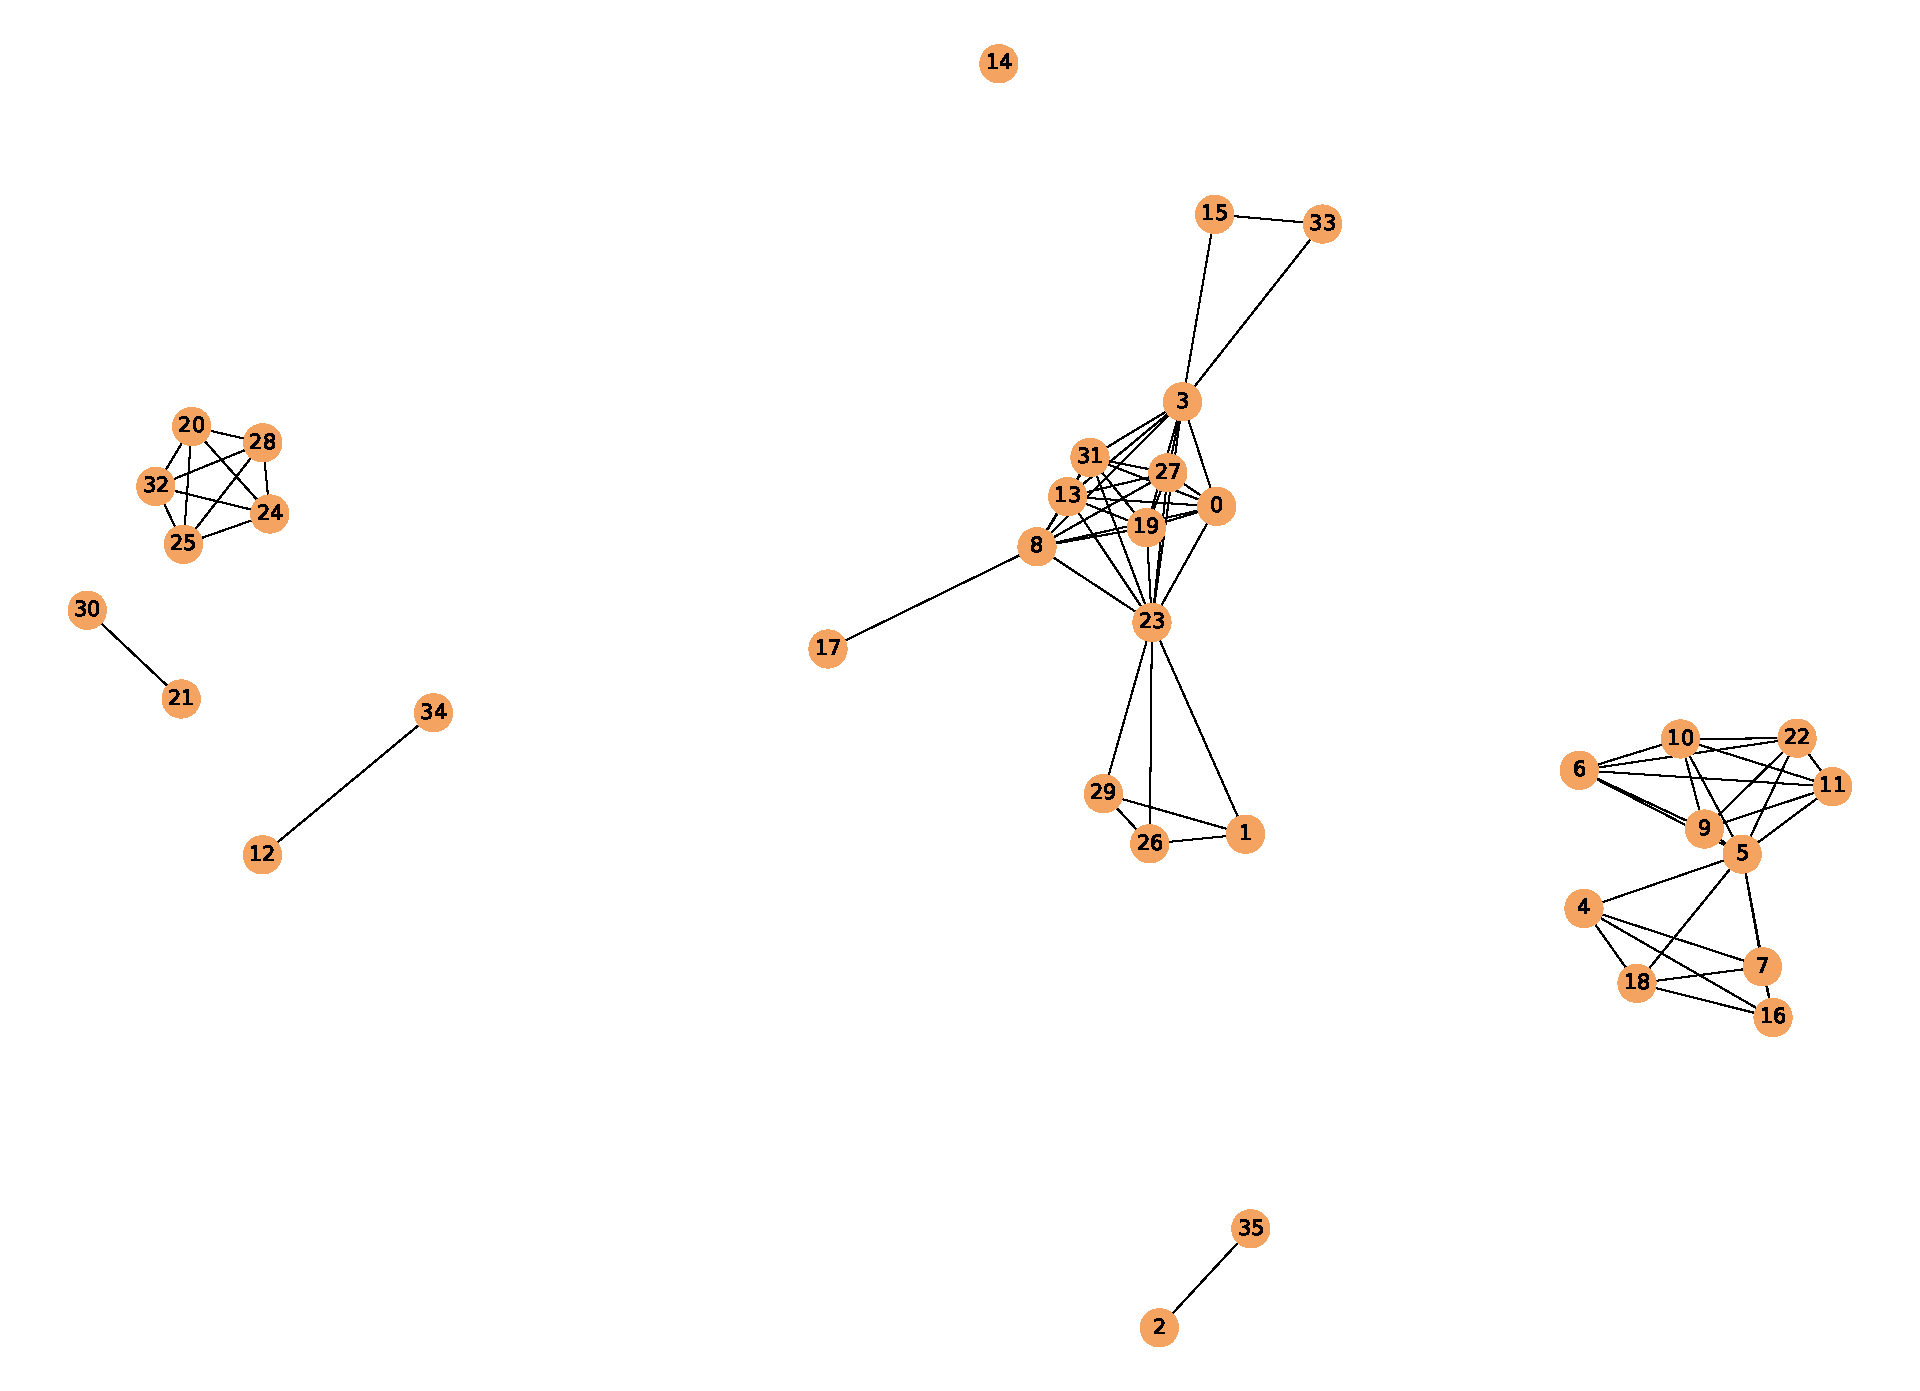
\includegraphics[width=\imsize]{Chap3/Proyecion_bipartita_ref_solo_tortus.pdf}
        \caption[Proyección  de red bipartita de refugios para datos de los tortugómetros en nodos tortuga.]{Proyección  de red bipartita de refugios para datos de los tortugómetros (Fig. \ref{fig:red_bipartita_refus_campanas}) en nodos tortuga. Si hay una refugio compartido por un par de nodos tortuga, aparece una conexión entre este par de nodos en la proyección. }
        \label{fig:proyeccion_red_campanas}
       
        \end{center}
\end{figure}
 
\begin{figure}[ht]
    \begin{center}
        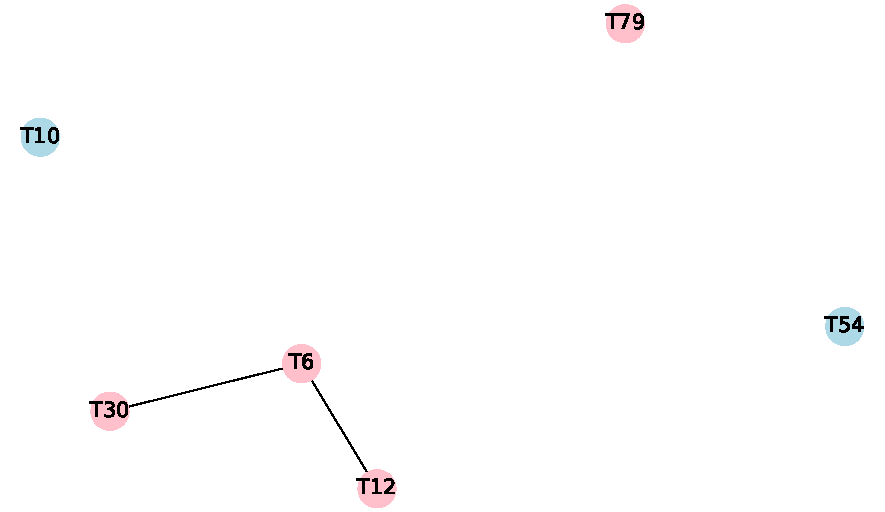
\includegraphics[width=\imsize]{Chap3/Proyecion_bipartita_ref_solo_tortus_IGOTU.pdf}
        \caption[Proyección  de red bipartita de refugios para datos de los tortugómetros en nodos tortuga.]{Proyección  de red bipartita de refugios para datos de los i-gotU (Fig. \ref{fig:red_bipartita_refus_igotu}) en nodos tortuga. Si hay una refugio compartido por un par de nodos tortuga, aparece una conexión entre este par de nodos en la proyección. }
        \label{fig:proyeccion_red_igotu}
       
        \end{center}
\end{figure}
Para  ver que tan probable es el encuentro entre tortugas, en caso que hayan usado alguna vez el mismo refugio, se decidió tomar las proyecciones de las redes bipartitas como predictores de conexiones en las redes de encuentros. Se calcularon las métricas precisión, accuracy y recall, partiendo de las cantidades verdadero positivo (TP), verdadero negativo (TN), falso positivo (FP) y falso negativo (FN). Donde, por ejemplo, TP se calculó como la cantidad de conexiones existentes en las redes de encuentros que también están en las redes proyectadas. La precisión se calculó como TP/(TP+FP), accuracy como (TP+TN)/(TP+TN+FP+FN) y  recall como TP/(TP+FN). Los resultados se muestran en la tabla \ref{tab:metricas_comparacion_redes}.
 
\begin{table}[ht]
    \centering
    \begin{tabular}{|c|c|c|c|}
       
   \hline
    Metodología  & Precisión & Recall & Accuracy \\ \hline
    Tortugómetro & 0.125     & 0.059  & 0.258    \\ \hline
    i-gotU       & 1         & 0.4    & 0.4       \\ \hline
   
    \end{tabular}
    \caption[Tabla con métricas de comparación entre redes de encuentros y proyecciones de redes bipartitas.]{Tabla con métricas de comparación entre redes de encuentros y proyecciones de redes bipartitas. Se tomó la proyección de la red bipartita como predictor de conexiones en las red de encuentros.}
    \label{tab:metricas_comparacion_redes}
\end{table}
 
Se observa en la tabla \ref{tab:metricas_comparacion_redes}, que las métricas obtenidas para los datos provenientes de los tortugómetros son considerablemente menores que las métricas obtenidas para los datos provenientes de los i-gotU. Estas diferencias se cree que están asociadas a la poca cantidad de refugios nocturnos medidos para los datos del tortugómetro, ya que originalmente las campañas de medición no se planearon para este tipo de análisis. Por otro lado, con los i-gotU se monitorean una menor cantidad de tortugas, produciendo una desviación en la medición.
 
Para determinar si los resultados de la tabla \ref{tab:metricas_comparacion_redes} son estadísticamente significativos, se realizaron operaciones de \textit{double edge swap} \cite{bipartitasTortusPaper} sobre las redes bipartitas de refugios y tortugas, y se compararon los valores obtenidos sobre estas nuevas redes generadas, después de haber hecho las proyecciones. Las redes generadas tenían la misma distribución de grado que las redes originales pero eran aleatorias con respecto a otras propiedades de las mismas y permiten comparar las métricas halladas con un modelo de correlación nula.
 
Se realizó un código en Python que elige dos conexiones al azar en la red bipartita y las intercambia, si es que no existen ya estas conexiones. Es decir, si T10 usó el refugio 54 y T11 el refugio 32, se intercambian los enlaces en caso que T10 no tenga una conexión con el refugio 32 y tampoco la T11 con el refugio 54 \cite{github}. Este procedimiento se itera de manera que genera una red aleatoria manteniendo la distribución de grado constante (un equivalente en cierto sentido a mantener la misma cantidad de mediciones pero tomando uso de refugios al azar). Partiendo de 1000 redes generadas a partir de 1000 cambios aleatorios de conexiones (1000 instancias de \textit{double edge swap}), se obtuvieron las métricas de precisión, recall y accuracy para cada red generada. Sobre estos valores se calculó la cantidad de veces donde las métricas halladas por usos aleatorios de refugios fueron mayores que los valores obtenidos  en la tabla \ref{tab:metricas_comparacion_redes}. Los resultados en términos de porcentajes donde se obtuvieron métricas mayores para cada metodología se muestran en la tabla \ref{tab:metricas_comparacion_redes_aleatorias}.
\begin{table}[ht]
    \centering
    \begin{tabular}{|c|c|c|c|}
       
   \hline
    Metodología  & \% Precisión mayor  &  \% Recall mayor & \% Accuracy mayor \\ \hline
    Tortugómetro & 60    & 50  & 50    \\ \hline
    i-gotU       & 0        & 0    & 0      \\ \hline
   
    \end{tabular}
    \caption[Tabla con comparación de métricas obtenidas en redes bipartitas con usos aleatorios de refugios respecto a las métricas medidas.]{Tabla con comparación de métricas obtenidas por redes bipartitas con usos aleatorios de refugios respecto de las métricas medidas. Se tomaron las proyecciones de la redes bipartitas generadas aleatoriamente como predictor de conexiones en las redes de encuentros y se calcularon las proporciones donde estas métricas son mayores a las obtenidas por la tabla \ref{tab:metricas_comparacion_redes}.}
    \label{tab:metricas_comparacion_redes_aleatorias}
\end{table}
 
Se observa en la tabla \ref{tab:metricas_comparacion_redes_aleatorias}, que las métricas obtenidas para los datos provenientes de los i-gotU son siempre mayor o iguales a lo esperado por uso aleatorio de refugios, mientras que las métricas obtenidas para los datos provenientes de los tortugómetros no lo son (es igual de probable obtener métricas mayores o menores mediante el uso aleatorio de refugios nocturnos). Esto se debe a que la cantidad de refugios nocturnos medidos para los datos del tortugómetro es considerablemente menor que la cantidad de refugios nocturnos medidos para los datos de los i-gotU. Por otro lado, con los i-gotU se monitorea una menor cantidad de tortugas, haciendo posible la existencia de un desvío de medición.
 
Una posible comparación entre las proyecciones de las redes bipartitas con las redes de encuentros está dada por la topología de las mismas.  En la siguiente sección se analiza la topología de las redes de encuentros y se compara con la topología de las redes proyectadas en nodos tortuga, comparando con métricas a partir del uso aleatorio de los refugios.
\section{Comparación topológica de redes de encuentros y redes proyectadas}
Se calcularon las métricas modularidad, densidad de la red, coeficiente de agrupamiento y centralidad de grado medio en nodos tortuga machos y hembras para las redes de encuentros (Figs. \ref{fig:redInteraccion20mincampanas} y \ref{fig:redInteraccion20igotu}) y para las redes proyectadas (Figs. \ref{fig:proyeccion_red_campanas} y \ref{fig:proyeccion_red_igotu}). En la tabla \ref{tab:metricas_topologia_redes}   se muestran los valores obtenidos para las distintas métricas, para los datos provenientes de las dos metodologías.
 
 
 
\begin{table}[ht]
    \centering
    \begin{tabular}{|c|c|c|c|c|}
    \hline
    Métricas          & E. Tortu   & P. Tortu      & E. i-gotU   & P. i-gotU    \\ \hline
    Modularidad       & 0,5         & 0,6           & 0,1        & 0            \\ \hline
    C. agrupamiento & 0,28        & 0,16          & 0           & 0            \\ \hline
    Densidad          & 0,22        & 0,09          & 0,50         & 0,13          \\ \hline
    C.G.M. machos     & $0.2\pm0.1$ & $0.08\pm0.08$ & $0.5\pm0.2$ & 0            \\ \hline
    C.G.M. hembras    & $0.2\pm0.1$ & $0.10\pm0.07$ & 0,5         & $0.2\pm0.1 $ \\ \hline
    \end{tabular}
    \caption[Tabla con métricas asociadas a las tipologías de las redes de encuentros y las redes proyectadas.]{Tabla con métricas asociadas a las topologías de las redes de encuentros y las redes proyectadas. E. y P. se refiere a redes de encuentros y redes proyectadas respectivamente, para cada metodología de medición. C. agrupamiento se refiere a coeficiente de agrupamiento y C.G.M. se refiere a centralidad de grado medio.}
    \label{tab:metricas_topologia_redes}
\end{table}
Podría esperarse que la centralidad de grado medio de los machos sea mayor que la de las hembras en base de observaciones de campo, especialmente en época de apareamiento (Nov-Dic), pero se encontró en la tabla \ref{tab:metricas_topologia_redes} que no presentan diferencias significativas para los datos provenientes de ambas metodologías \cite{Erika}. Se encontró menor densidad de red en la red proyectada de tortugas que en la red de encuentros, para ambas metodologías. Esto está relacionado con la poca cantidad de mediciones de refugios compartidos. En el caso de los tortugómetros, el filtro para la selección de refugios es muy estricto, generando una poca cantidad de refugios respecto de la cantidad de días de medición. Por otro lado, en el caso de los i-gotU, la cantidad de refugios medidos es alta pero la mayoría de estos fueron medidos en meses donde la tortuga baja la actividad a causa de las temperaturas del ambiente y decide quedarse la mayor parte de las noches en los refugios preferidos encontrados (Fig. \ref{fig:refugios_preferidos}).
 
Con respecto al coeficiente de agrupamiento, se observa que para los datos provenientes de los tortugómetros, el coeficiente de agrupamiento es distinto de cero. Para el caso de los datos provenientes de los i-gotU, el coeficiente de agrupamiento es cero. Esto se debe a que la red de encuentros y la red proyectada no presentan triángulos entre ningún triplete de nodos, debido seguramente a la poca cantidad de individuos monitoreados con este método.
 
Se utilizó la modularidad para detectar la fuerza de unión en comunidades en la red. Se detectaron la existencia de dos claras comunidades en las redes provenientes de los datos del tortugómetro (Figs. \ref{fig:redInteraccion20mincampanas} y \ref{fig:proyeccion_red_campanas}) y a la ausencia de comunidades en las redes de los datos de los i-gotU (Figs. \ref{fig:redInteraccion20igotu} y \ref{fig:proyeccion_red_igotu}).
 
Para comparar las métricas obtenidas con un modelo de uso aleatorio de refugios, se generaron 1000 redes aleatorias  realizando 1000 operaciones del tipo \textit{double edge swap} sobre las redes bipartitas. Se compararon las métricas obtenidas en las redes proyectadas de la tabla \ref{tab:metricas_topologia_redes} con las métricas obtenidas en las proyecciones de las redes aleatorias. En la Fig. \ref{fig:distribucion_coef_agrupa}, se muestra un ejemplo de la distribución del coeficiente de agrupamiento en las redes aleatorias generadas partiendo de la red bipartita de refugios con datos de los tortugómetros (Fig. \ref{fig:red_bipartita_refus_campanas}). Se observa que no presenta diferencias significativas entre los valores hallados con el valor medido en la proyección de la red original. Se observó el mismo tipo de comportamiento para todas las métricas calculadas en la tabla \ref{tab:metricas_topologia_redes}. Esto quiere decir que no habría diferencias con una red aleatoria y que por lo tanto no parece ser posible inferir información de una red de a partir de la otra.
\begin{figure}[ht]
    \begin{center}
        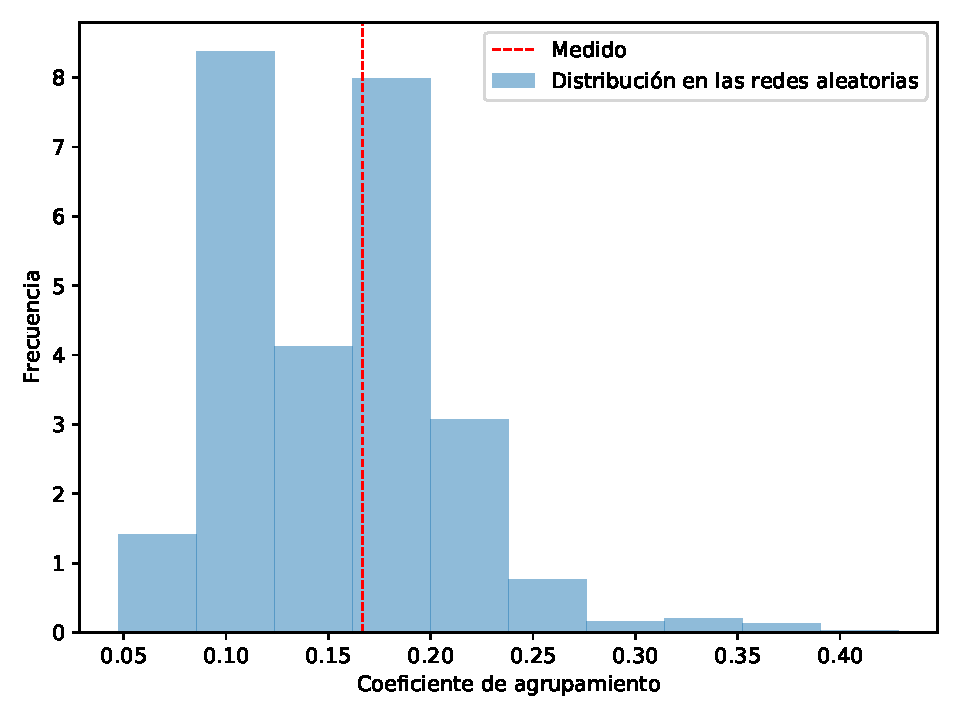
\includegraphics[width=\imsize]{Chap3/coef_clustering_distribucion.pdf}
        \caption[Distribución del coeficiente de agrupamiento en proyecciones de redes aleatorias.]{Distribución del coeficiente de agrupamiento calculado de las proyecciones en nodos tortuga de mil redes generadas aleatoriamente a partir de la red bipartita con datos de los tortugómetros. En rojo está el valor medido del coeficiente de agrupamiento para la proyección en nodos tortuga (Fig. \ref{fig:proyeccion_red_campanas}).}
        \label{fig:distribucion_coef_agrupa}
       
        \end{center}
\end{figure}
 
\section{Proyecciones de redes bipartitas en nodos refugio}
Se realizaron las proyecciones de las redes bipartitas (Figs. \ref{fig:red_bipartita_refus_campanas} y \ref{fig:red_bipartita_refus_igotu}) en nodos refugio, Figs. \ref{fig:proyeccion_red_campanas_refus} y \ref{fig:proyeccion_red_igotu_refus}.
 
 
\begin{figure}[ht]
    \begin{center}
        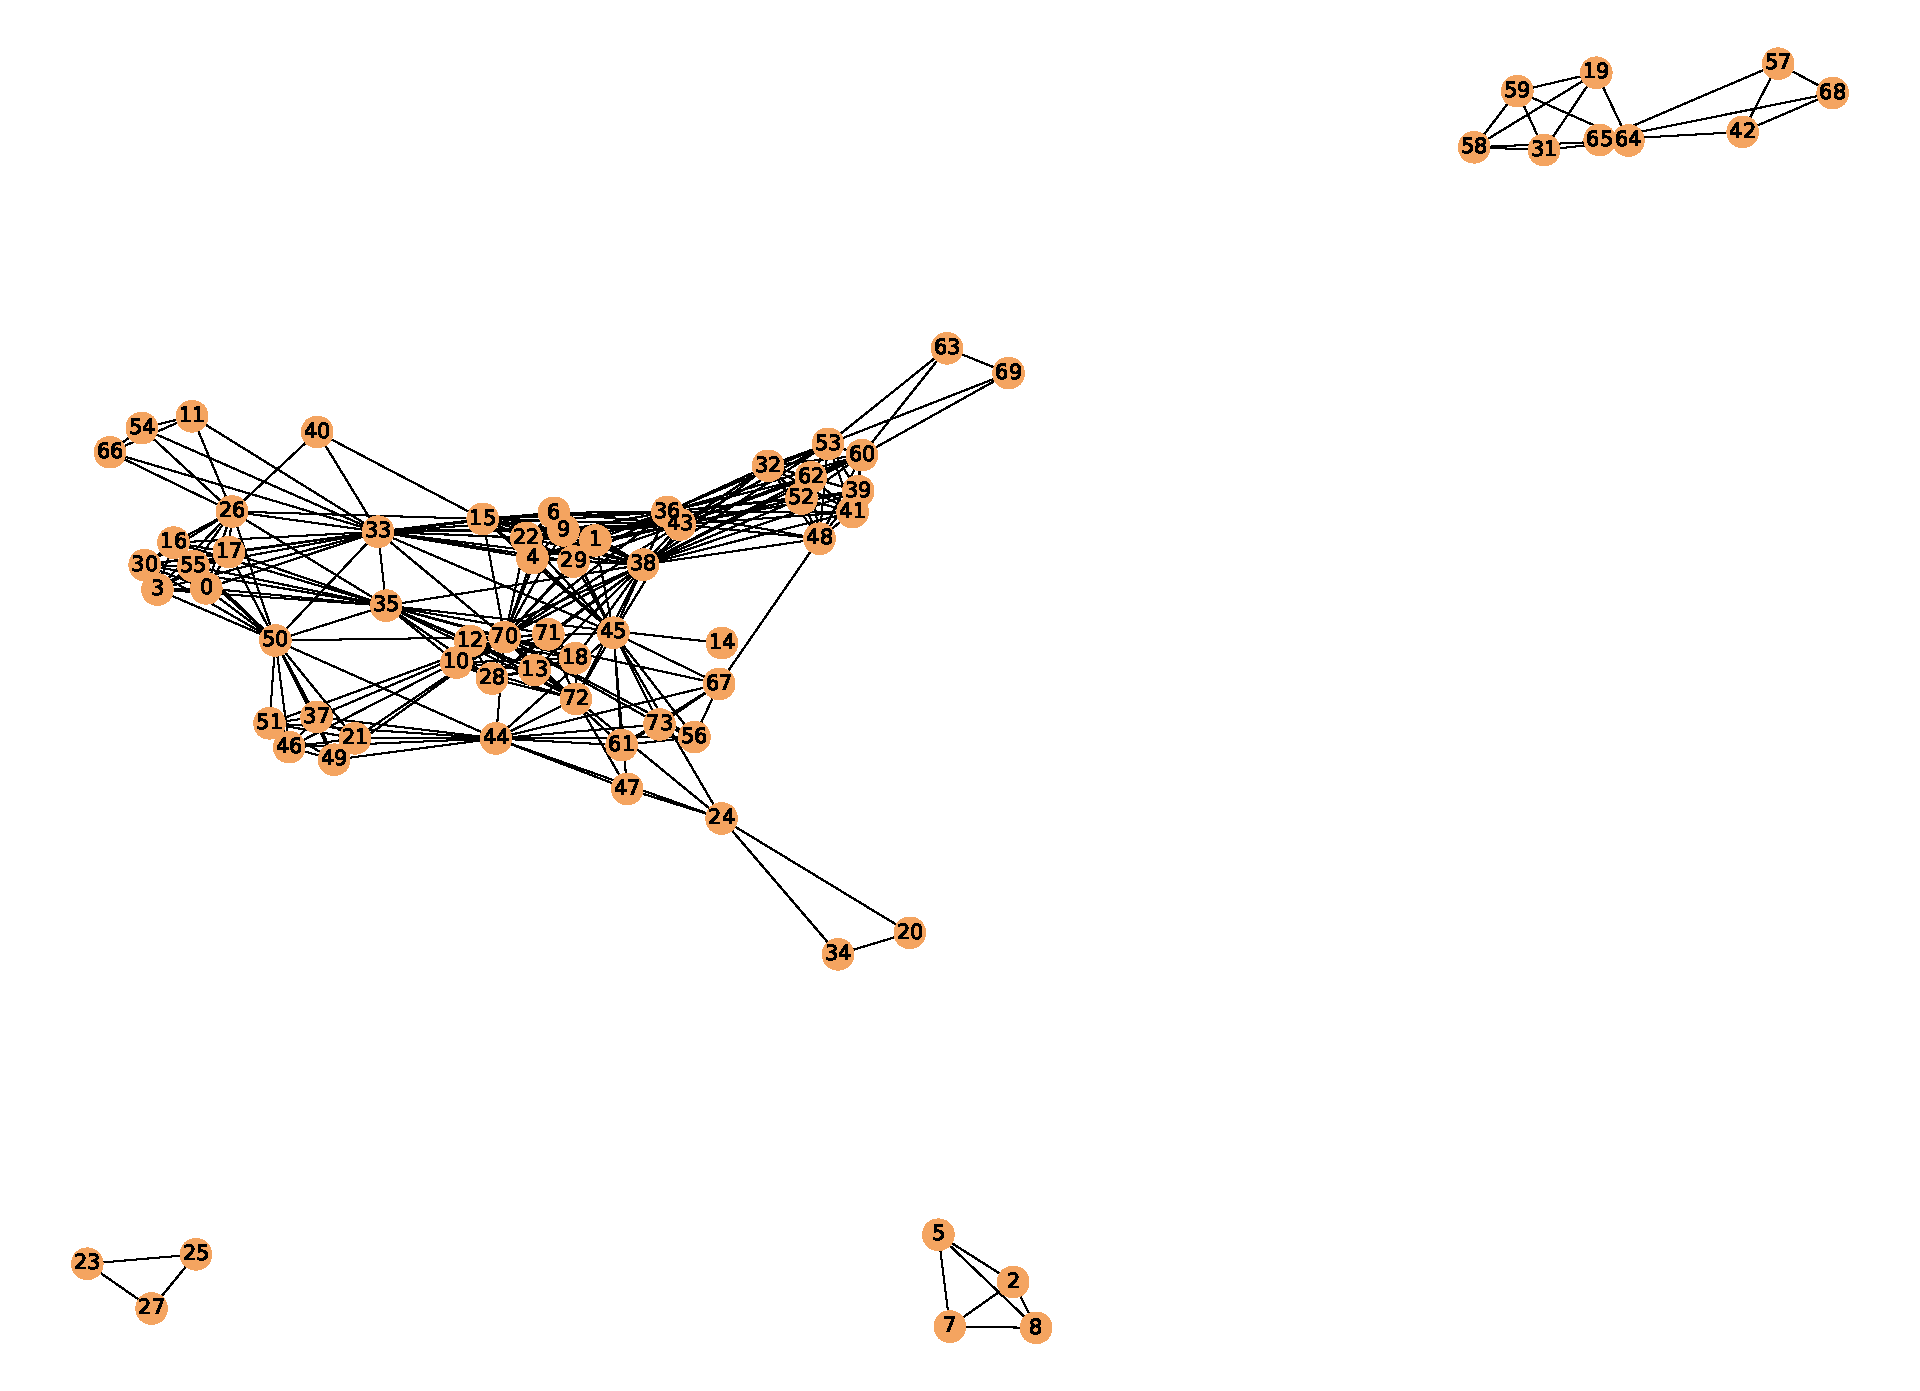
\includegraphics[width=\imsize]{Chap3/Proyecion_bipartita_ref_solo_ref.pdf}
        \caption[Proyección  de red bipartita de refugios para datos de los tortugómetros en nodos refugio.]{Proyección  de red bipartita de refugios para datos de los tortugómetros (Fig. \ref{fig:red_bipartita_refus_campanas}). Si hay un refugio compartido por un par de nodos tortuga, aparece una conexión entre este par de nodos en la proyección. }
        \label{fig:proyeccion_red_campanas_refus}
       
        \end{center}
\end{figure}
 
\begin{figure}[ht]
    \begin{center}
        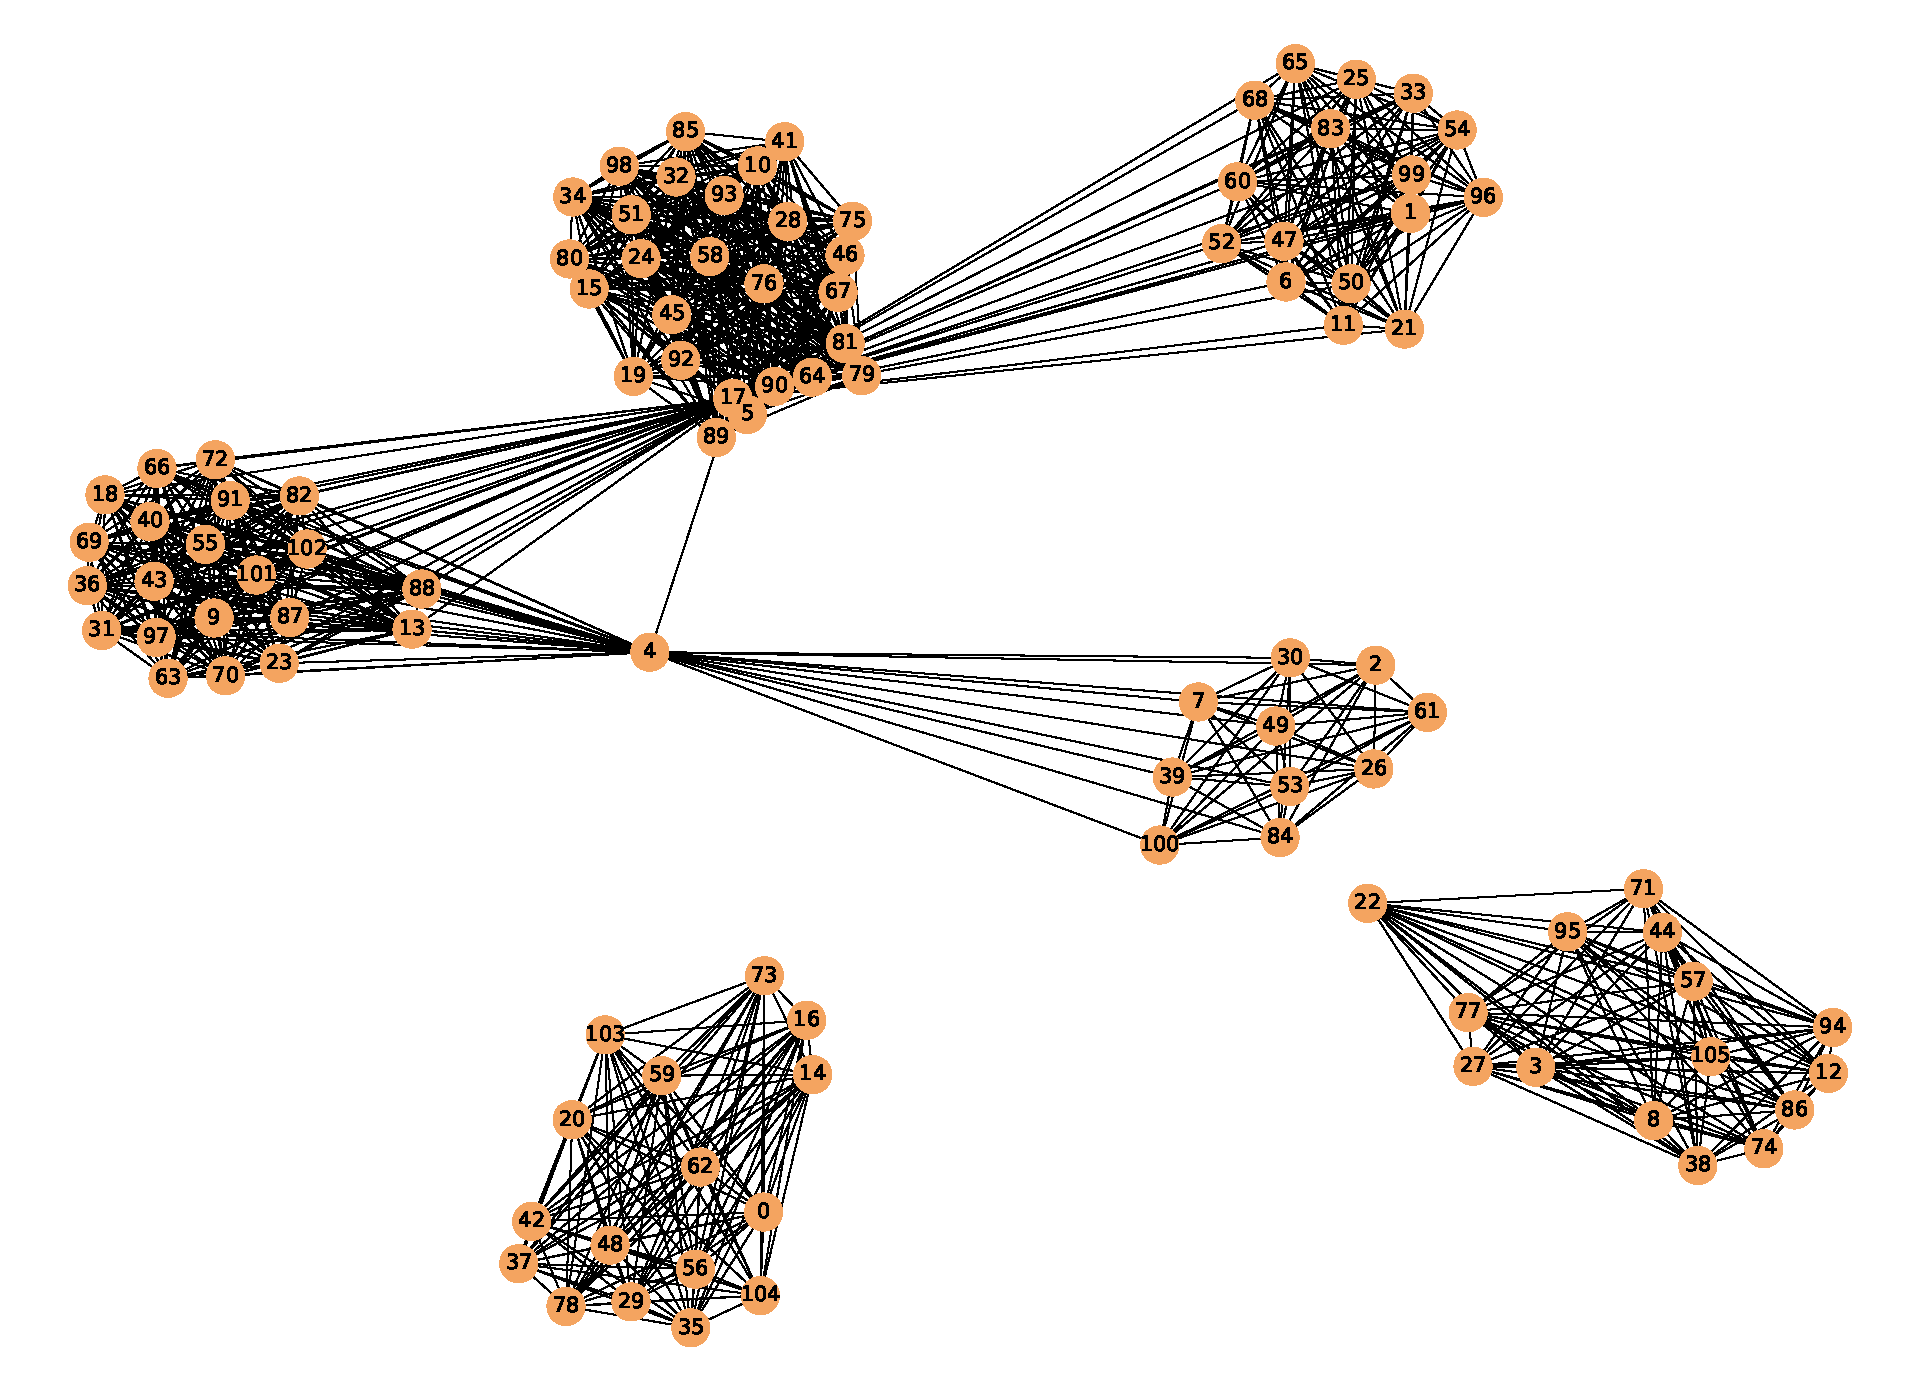
\includegraphics[width=\imsize]{Chap3/Proyecion_bipartita_ref_solo_ref_iGOTU.pdf}
        \caption[Proyección  de red bipartita de refugios para datos de los i-gotU en nodos refugio.]{Proyección  de red bipartita de refugios para datos de los i-gotU (Fig. \ref{fig:red_bipartita_refus_igotu}) sobre los nodos refugio. Si hay un refugio compartido por un par de nodos tortuga, aparece una conexión entre el refugio común con los respectivos refugios de ambas tortugas en la proyección. }
        \label{fig:proyeccion_red_igotu_refus}
       
        \end{center}
\end{figure}
En las Figs. \ref{fig:proyeccion_red_campanas_refus} y \ref{fig:proyeccion_red_igotu_refus}, se observan pequeños clusters donde hay nodos completamente conectados (asociados a los refugios que visitó una tortuga) con algunos nodos que conectan distintos clusters (asociados a algún refugio compartido). Un ejemplo de este nodo conector es el refugio 4 (Fig. \ref{fig:proyeccion_red_igotu_refus}), que fue utilizado por la tortuga T30 y T6 en distintas noches (Fig. \ref{fig:red_bipartita_refus_igotu}).
 
Una pregunta subyacente de las proyecciones calculadas es si existe alguna relación entre los enlaces de la red y las distancias geográficas entre los nodos refugio. Para responder esta pregunta se graficaron los refugios en el mapa junto con las conexiones dadas por los enlaces en las proyecciones. Un ejemplo de este mapa para los datos de los i-gotU se muestra en la Fig. \ref{fig:mapa_con_conexiones_igotu}. Se observa que parte de los enlaces se encuentran entre refugios vecinos, pero también hay unos pocos enlaces entre refugios que se encuentran a distancias considerables respecto de refugios vecinos. A falta de una relación más rigurosa entre las distancias y los enlaces, se realizó un \textit{Mantel test} \cite{MantelTest} entre las matrices de adyacencia de las redes proyectadas en nodos refugio (Figs. \ref{fig:proyeccion_red_campanas_refus} y \ref{fig:proyeccion_red_igotu_refus}) con matrices de distancias entre refugios. La matriz de adyacencia está definida como la matriz booleana que representa las conexiones entre pares de nodos refugio. En el lugar $i$,$j$ de la matriz de distancias se encuentra la distancia entre el refugio  de la posición $i$ y el refugio $j$ (en metros) de la matriz de adyacencia.
 
El Mantel test calcula el coeficiente de correlación de Pearson entre estas dos matrices, luego realiza permutaciones aleatorias de la matriz de distancias y vuelve a calcular el coeficiente de correlación de Pearson. El p-valor es la proporción de permutaciones que dan un coeficiente de correlación de Pearson mayor o igual al coeficiente de correlación de Pearson de la matriz de distancias original. Bajo la hipótesis de correlación nula en las dos matrices, las permutaciones aleatorias deberían ser igualmente probables de producir valores mayores o menores del coeficiente de correlación calculado.
 
 
Los Mantel tests realizados con 10000 permutaciones aleatorias para los datos de los tortugómetros y los i-gotU dan un p-valor de 0.0051 y 0.0001 respectivamente. Esto indica que existe una correlación significativa entre las distancias entre refugios y los enlaces en las redes proyectadas en nodos refugio (Figs. \ref{fig:proyeccion_red_campanas_refus} y \ref{fig:proyeccion_red_igotu_refus}). Es decir que la tortuga que visita un refugio tiene una probabilidad mayor de visitar refugios cercanos a este, como se observa en la Fig. \ref{fig:mapa_con_conexiones_igotu}. Esto también se evidencia observando la trayectoria de visita de los refugios, siendo la regla que la tortuga posee noches consecutivas en refugios cercanos entre sí (Fig. \ref{fig:ruta_refus_T54}).
 
\begin{figure}[ht]
    \begin{center}
        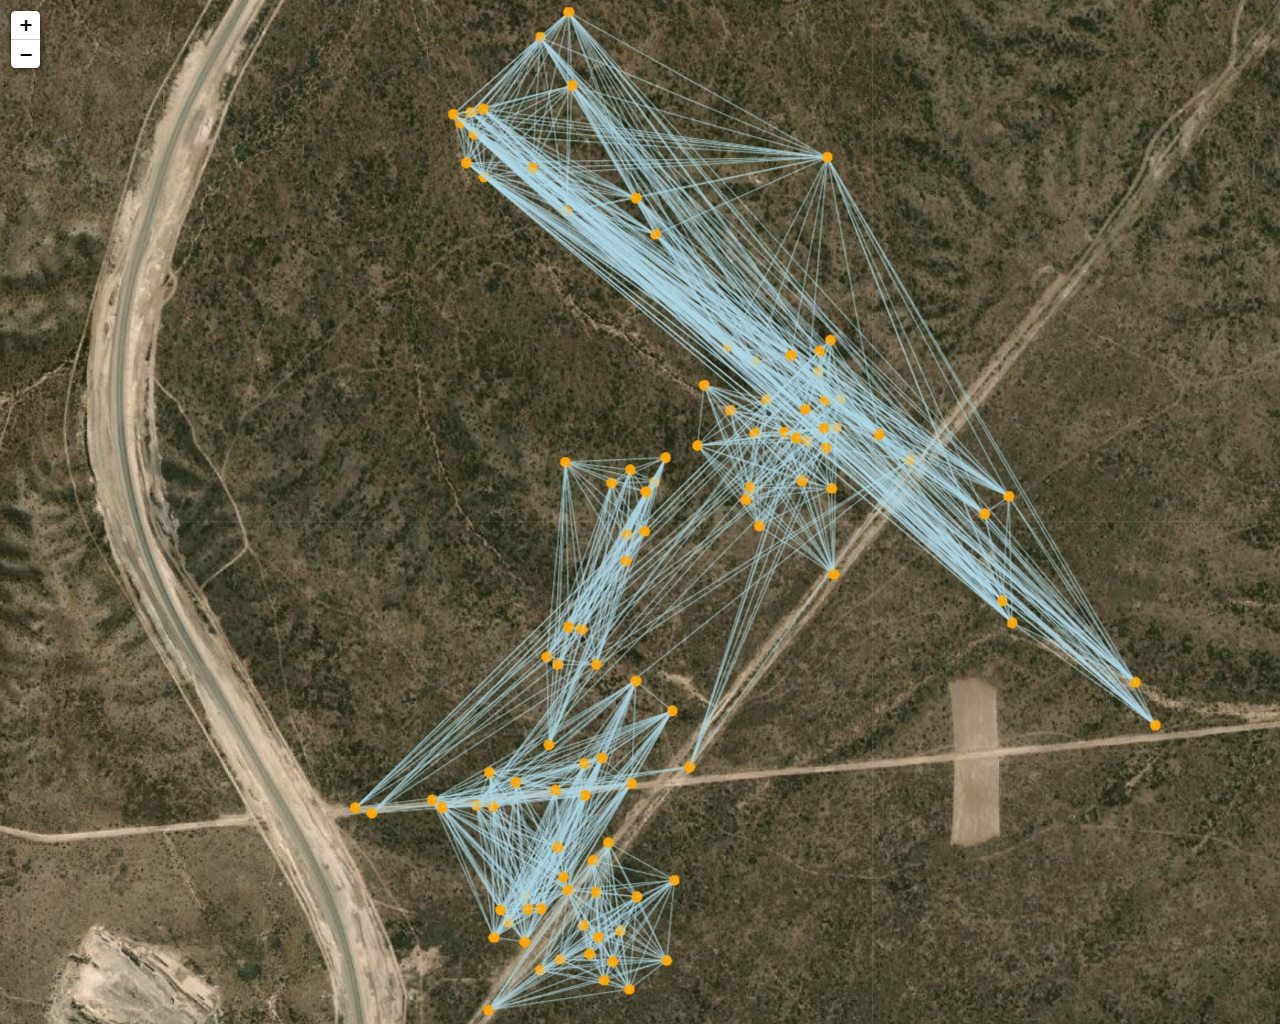
\includegraphics[width=\imsize]{Chap3/Mapa_refus_con_coneciones_igotu.jpg}
        \caption[Proyección en nodos refugio con conexiones en el mapa.]{Proyección de red bipartita (Fig. \ref{fig:proyeccion_red_igotu_refus}) en nodos refugio con conexiones en el mapa para los datos de i-gotU. }
        \label{fig:mapa_con_conexiones_igotu}
       
        \end{center}
\end{figure}
 
 
 
 
 
 
 
 
 

